\documentclass[12pt]{article}
\usepackage[dvips]{epsfig}
\usepackage{color}
%e.g.  \textcolor{red,green,blue}{text}
\usepackage{url}
\usepackage[colorlinks=true]{hyperref}

\begin{document}

\section*{GENESIS: Documentation}

\section*{Part--II: Modeling Dendrites and Synapses}

In the Introduction to Computational Neuroscience, and Modeling of Action Potentials (link) we learned the basics of compartmental modeling of neurons, including the Hodgkin-Huxley models of voltage activated channels. In this lecture and the following one, we will talk about what goes on in the dendrites and how this relates to the behavior of more complex cells and networks.

The image of the pyramidal cell from the CA3 region of the hippocampus that we looked at in the last lecture is just one of the many varieties of neurons that one might want to model. Here are some others:

\begin{figure}[h]
  \centering
 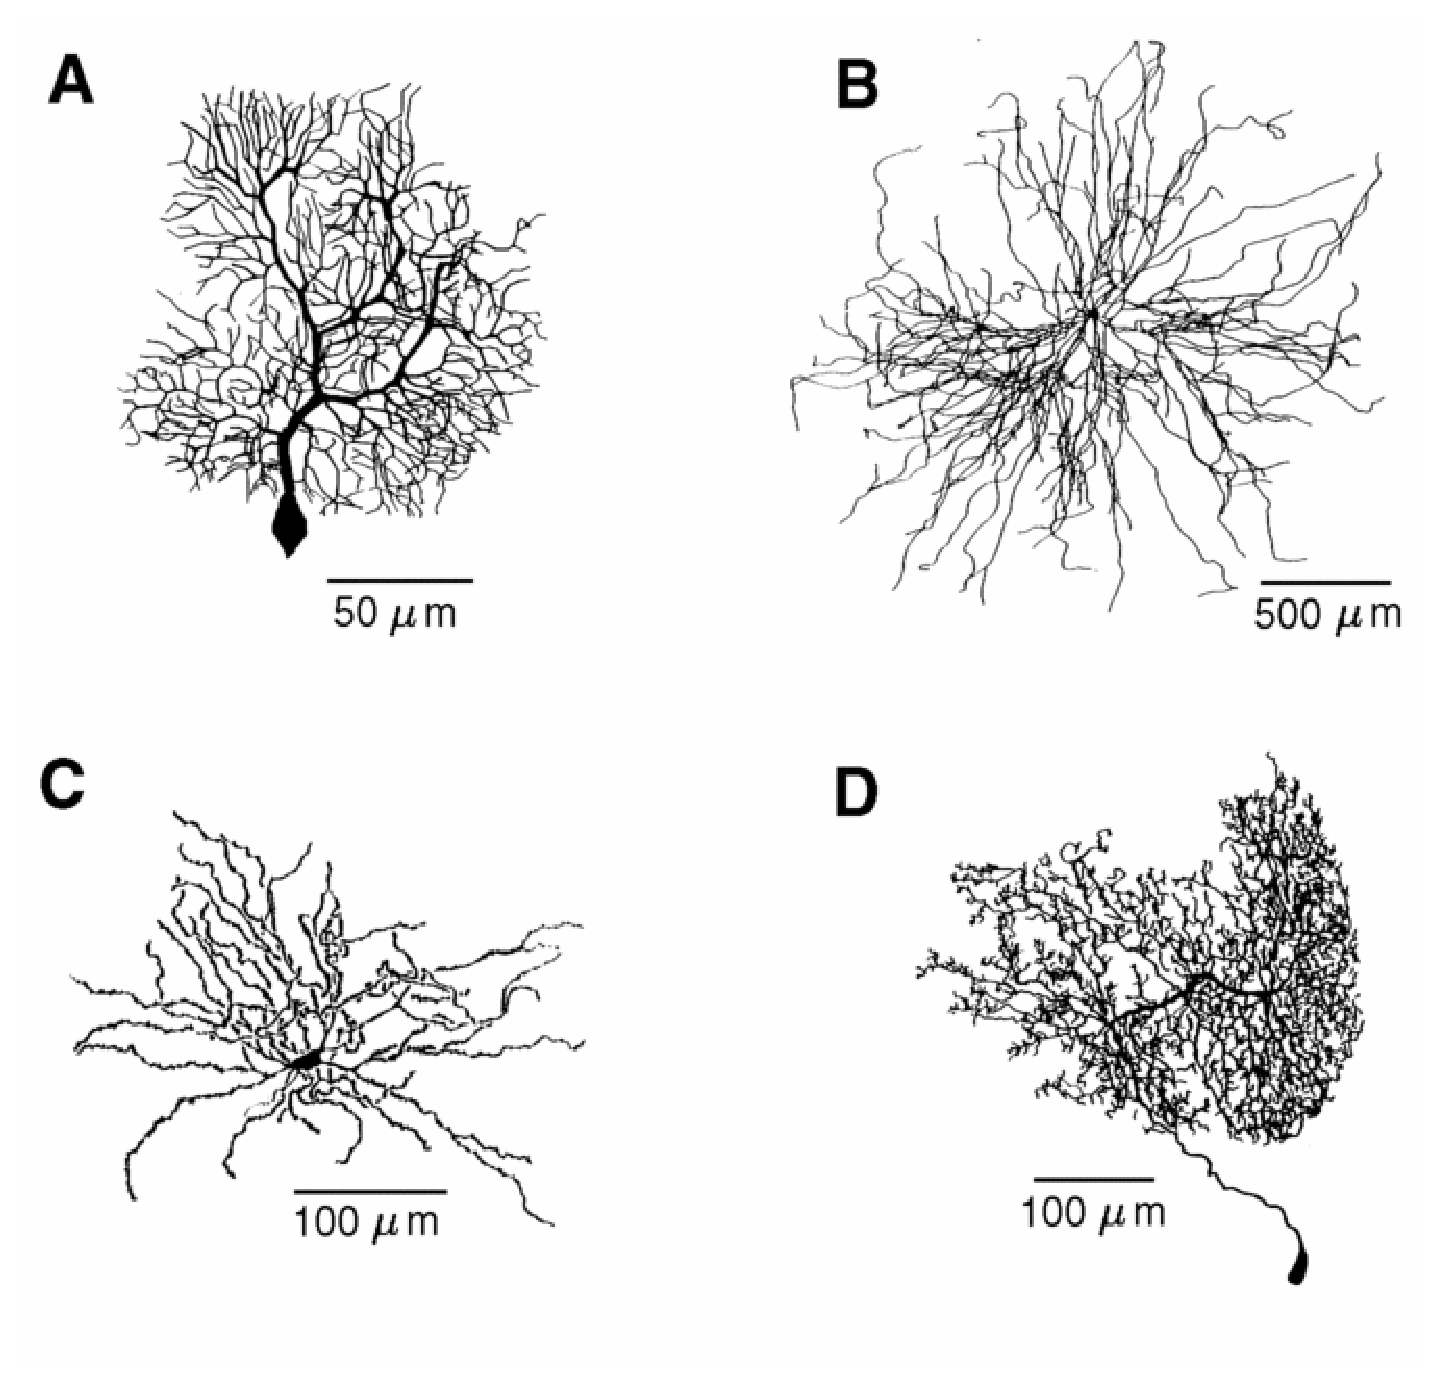
\includegraphics[scale=0.4]{figures/BoGfig5_1s.eps}
  \caption{(A) Cerebellar Purkinje cell; (B) spinal cord motoneuron; (C) neostriatal spiny neuron; (D) locust interneurons}
  \label{fig:neurons}
\end{figure}

The many varieties of dendritic structure that are seen in these cells has a great deal to do with their functional role--i.e., the types of ``neural computations" that are performed.

There are four main steps to perform in order to build a realistic model neuron, and to connect it to others in biologically realistic network.

\begin{enumerate}
\item Create a morphological reconstruction of the cell to be modeled. Neurons are stained, and a specialized microscope and software are used to trace the dendritic structure and create a data file with segment coordinates, lengths, diameters, and branch points.

\item Build a suitably realistic passive compartmental model, without the variable conductances. This may involve simplifications of the reconstruction. There are two main questions to be answered:

\begin{enumerate}
\item How long should a compartment be?

\item What values of $R_m$, $C_m$, and $R_a$ should be used for each compartment? 
\end{enumerate}

\item Add the appropriate variable conductances to compartments that correspond to the part of the cell where they appear.

\begin{enumerate}
\item Add voltage and/or calcium activated conductances. These are usually implemented with some variation of the Hodgkin-Huxley model described in the previous lecture, with parameters derived from voltage clamp data on neurons that contain the conductances to be modeled.

\item Add synaptically activated conductances, using a model to be covered a little later in this lecture. 
\end{enumerate}

\item Connect to other cells in a network, or provide artificial inputs to simulate the in-vivo inputs to the neuron.
\end{enumerate}

Step 2 is difficult. \href{../bog-ch5/bog-ch5.pdf}{Chapter 5} of {\it The Book of GENESIS} (``the BoG"), gives some useful information for answering the two questions. This chapter (Segev, 2005) is also very mathematical, and it is easy to get lost in the equations and forget what they are used for. You should read it in order to get an overview of the theory of passive propagation in dendrites. It is important to remember that there are three things that can be measured experimentally and are related to the parameters needed for a model:

\begin{enumerate}
\item The attentuation of voltage with distance, and the ``space constant" or ``length constant", lambda ($\lambda$).

\item The membrane time constant tau ($\tau$).

\item The input resistance of the cell ($R_m$), measured at the soma.
\end{enumerate}

This slide gives a summary of the electrical properties of a uniform section of passive dendrite having length $l$ and diameter $d$.

\begin{figure}[h]
  \centering
 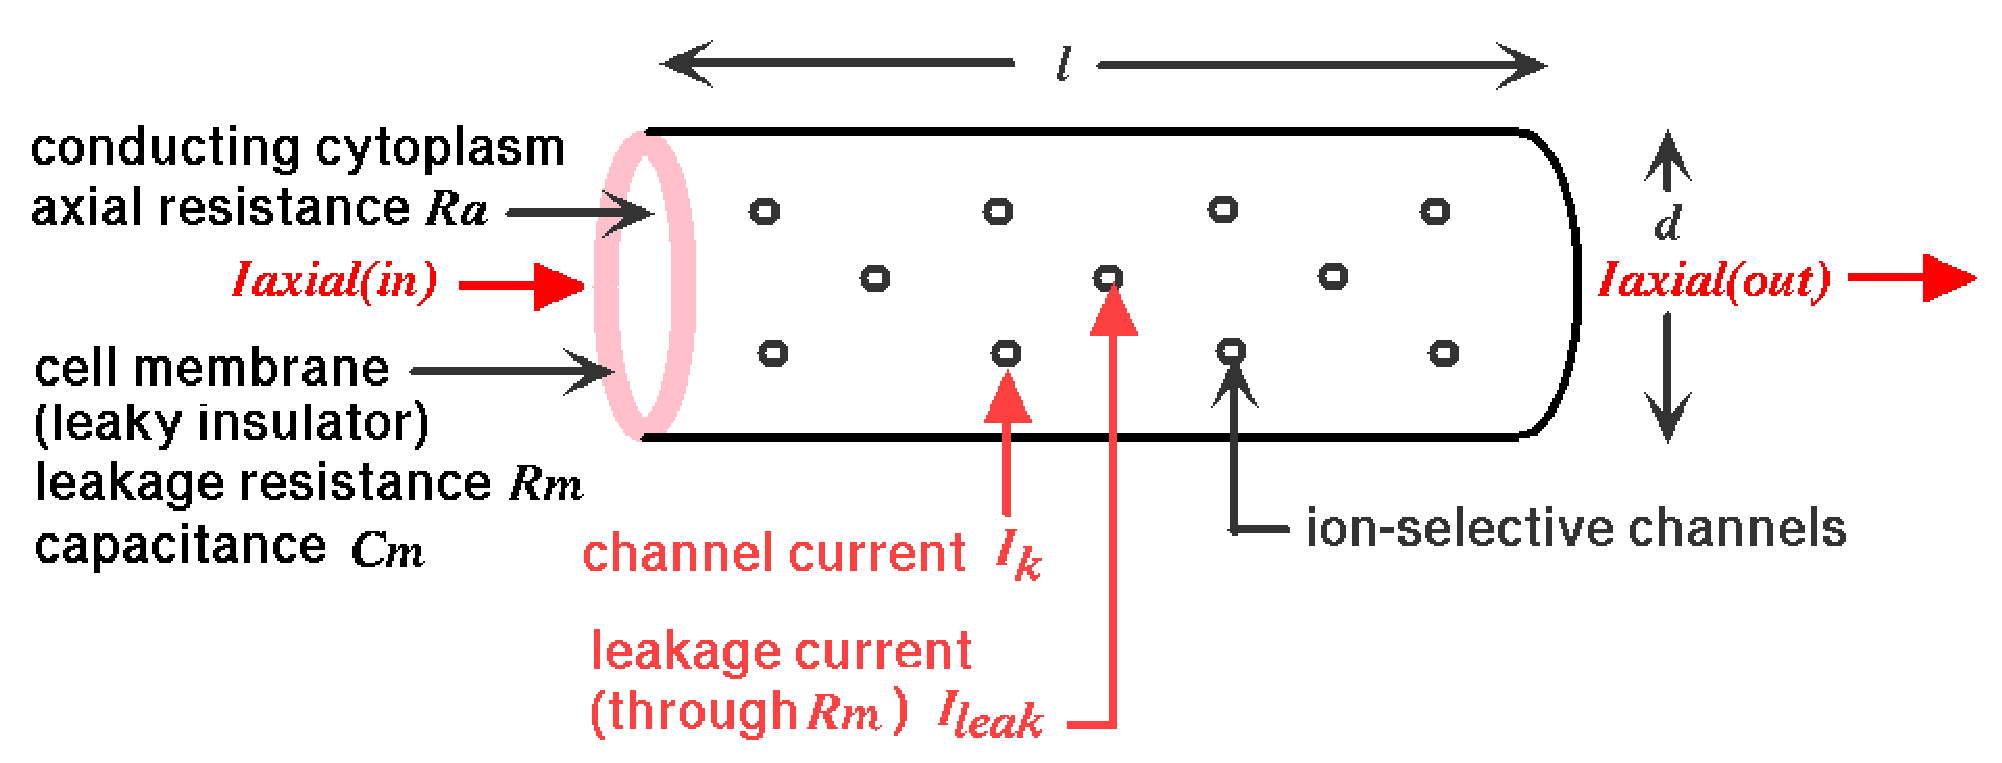
\includegraphics[scale=0.4]{figures/dendrite_section2.eps}
  %\caption{enumerate}
  \label{fig:dendrite2}
\end{figure}

The conducting cytoplasm inside the neuron, the insulating neural membrane, and the liquid (similar to salt water) surrounding the neuron form a cable with a capacitance$ C_m$. The inner conductor, the cytoplasm, is a poorer conductor than the copper wire used in an undersea cable, and it has an ``axial resistance" along its length, $R_a$. The membrane in not a perfect insulator due to the ion-conducting channels that pass through it. It is convenient to make a distinction between the ``passive channels" that do not vary in conductance, and the ``active channels" that have conductances varying with voltage, calcium concentration, or synaptic input. The passive channels account for the membrane resistance $R_m$ and the associated leakage current $I_{leak}$. The active channels are represented by the various variable conductances that are labeled as $G_k$ in the neural compartment diagram above and the differential equation for $V_m$ that we described in the Introduction to Computational Neuroscience(make link to G3-IntroCompNeurosci1.tex):

\begin{figure}[h]
  \centering
 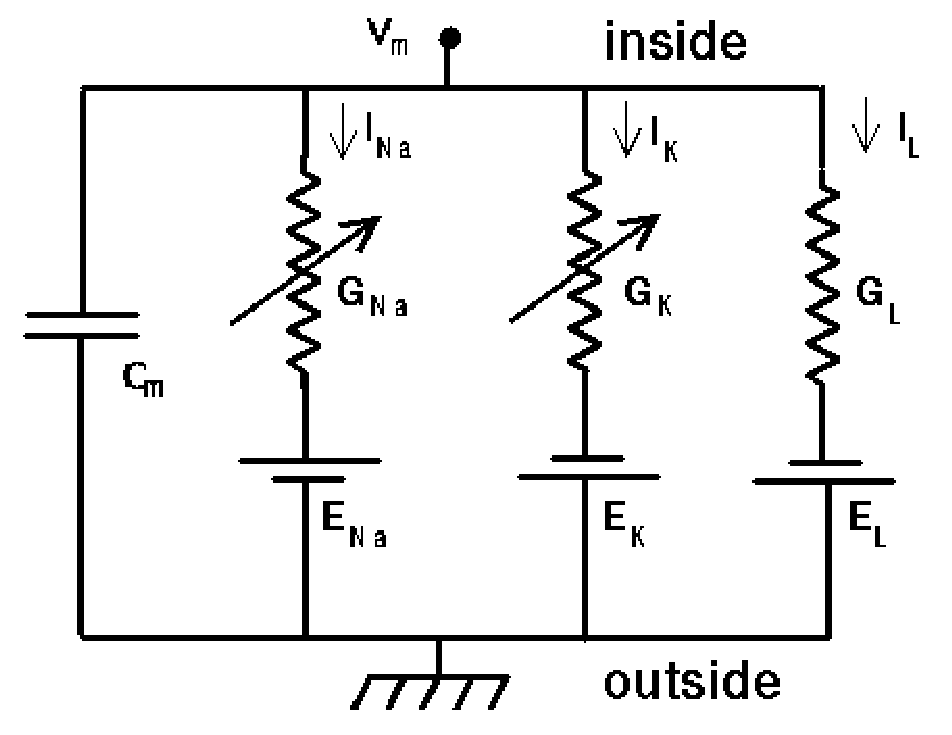
\includegraphics[scale=0.5]{figures/HHcompt.eps}
  %\caption{enumerate}
  \label{fig:dendrite}
  \begin{displaymath}
		C_m \frac{dV_m}{dt} = \frac{(E_m-V_m)}{R_m}+\sum_k [G_k(E_k-V_m)]+\frac{(V_m'-V_m)}{R_a'} + \frac{(V_m''-V_M)}{R_a} +I_{inject}
\label{eq:figeq1}		
\end{displaymath}
\end{figure}

\subsection*{Some Notation}

The quantities $R_m$, $R_a$, $C_m$, $V_m$, etc. that appear in the diagram and equation below are given in ohms, farads, or volts, respectively, and will depend on the size of the compartment. In order to specify parameters that are independent of the compartment dimensions, {\it specific units} are used. For a cylindrical compartment, the membrane resistance is inversely proportional to the area of the cylinder, so we define a {\it specific membrane resistance} $R_M$, which has units of ohms$\cdot$m$^2$. The membrane capacitance is proportional to the area, so it is expressed in terms of a {\it specific membrane capacitance} $C_M$, with units of farads/m$^2$. Compartments are connected to each other through their axial resistances Ra. The axial resistance of a cylindrical compartment is proportional to its length and inversely proportional to its cross-sectional area. Therefore, we define the {\it specific axial resistance} $R_A$ to have units of ohms/m.

For a piece of dendrite or a compartment of length $l$ and diameter $d$ we then have

\begin{displaymath}R_{m} = \frac{R_M}{\pi l d},\; C_{m} = \pi l d C_M,\; R_{a}= \frac{4 l R_A}{\pi d^{2}}. \end{displaymath}

\textcolor{red}{WARNING:} Many treatments of the passive properties of neural tissue use the symbols $R_m$, $R_a$, and $C_m$ for the specific resistances and capacitance, instead of this notation with $R_M$, $R_A$, and $C_M$. Also, many textbooks and journal papers define the resistance and capacitance in terms of that for a unit length of cable having a specified diameter.

Sections 5.3 through 5.5 in BoG \href{../bog-ch5/bog-ch5.pdf}{Chapter 5} describes how sections of dendrite can be modeled using the one-dimensional cable equation. For some additional background with more details than are given in this lecture, see the \href{../cable-theory}{Digression on Cable Theory of Passive Propagation in Dendrites}.

The relationships between the original neuron and a cable model or a compartmental models are shown in BoG Figure 5.4:

\begin{figure}[h]
  \centering
 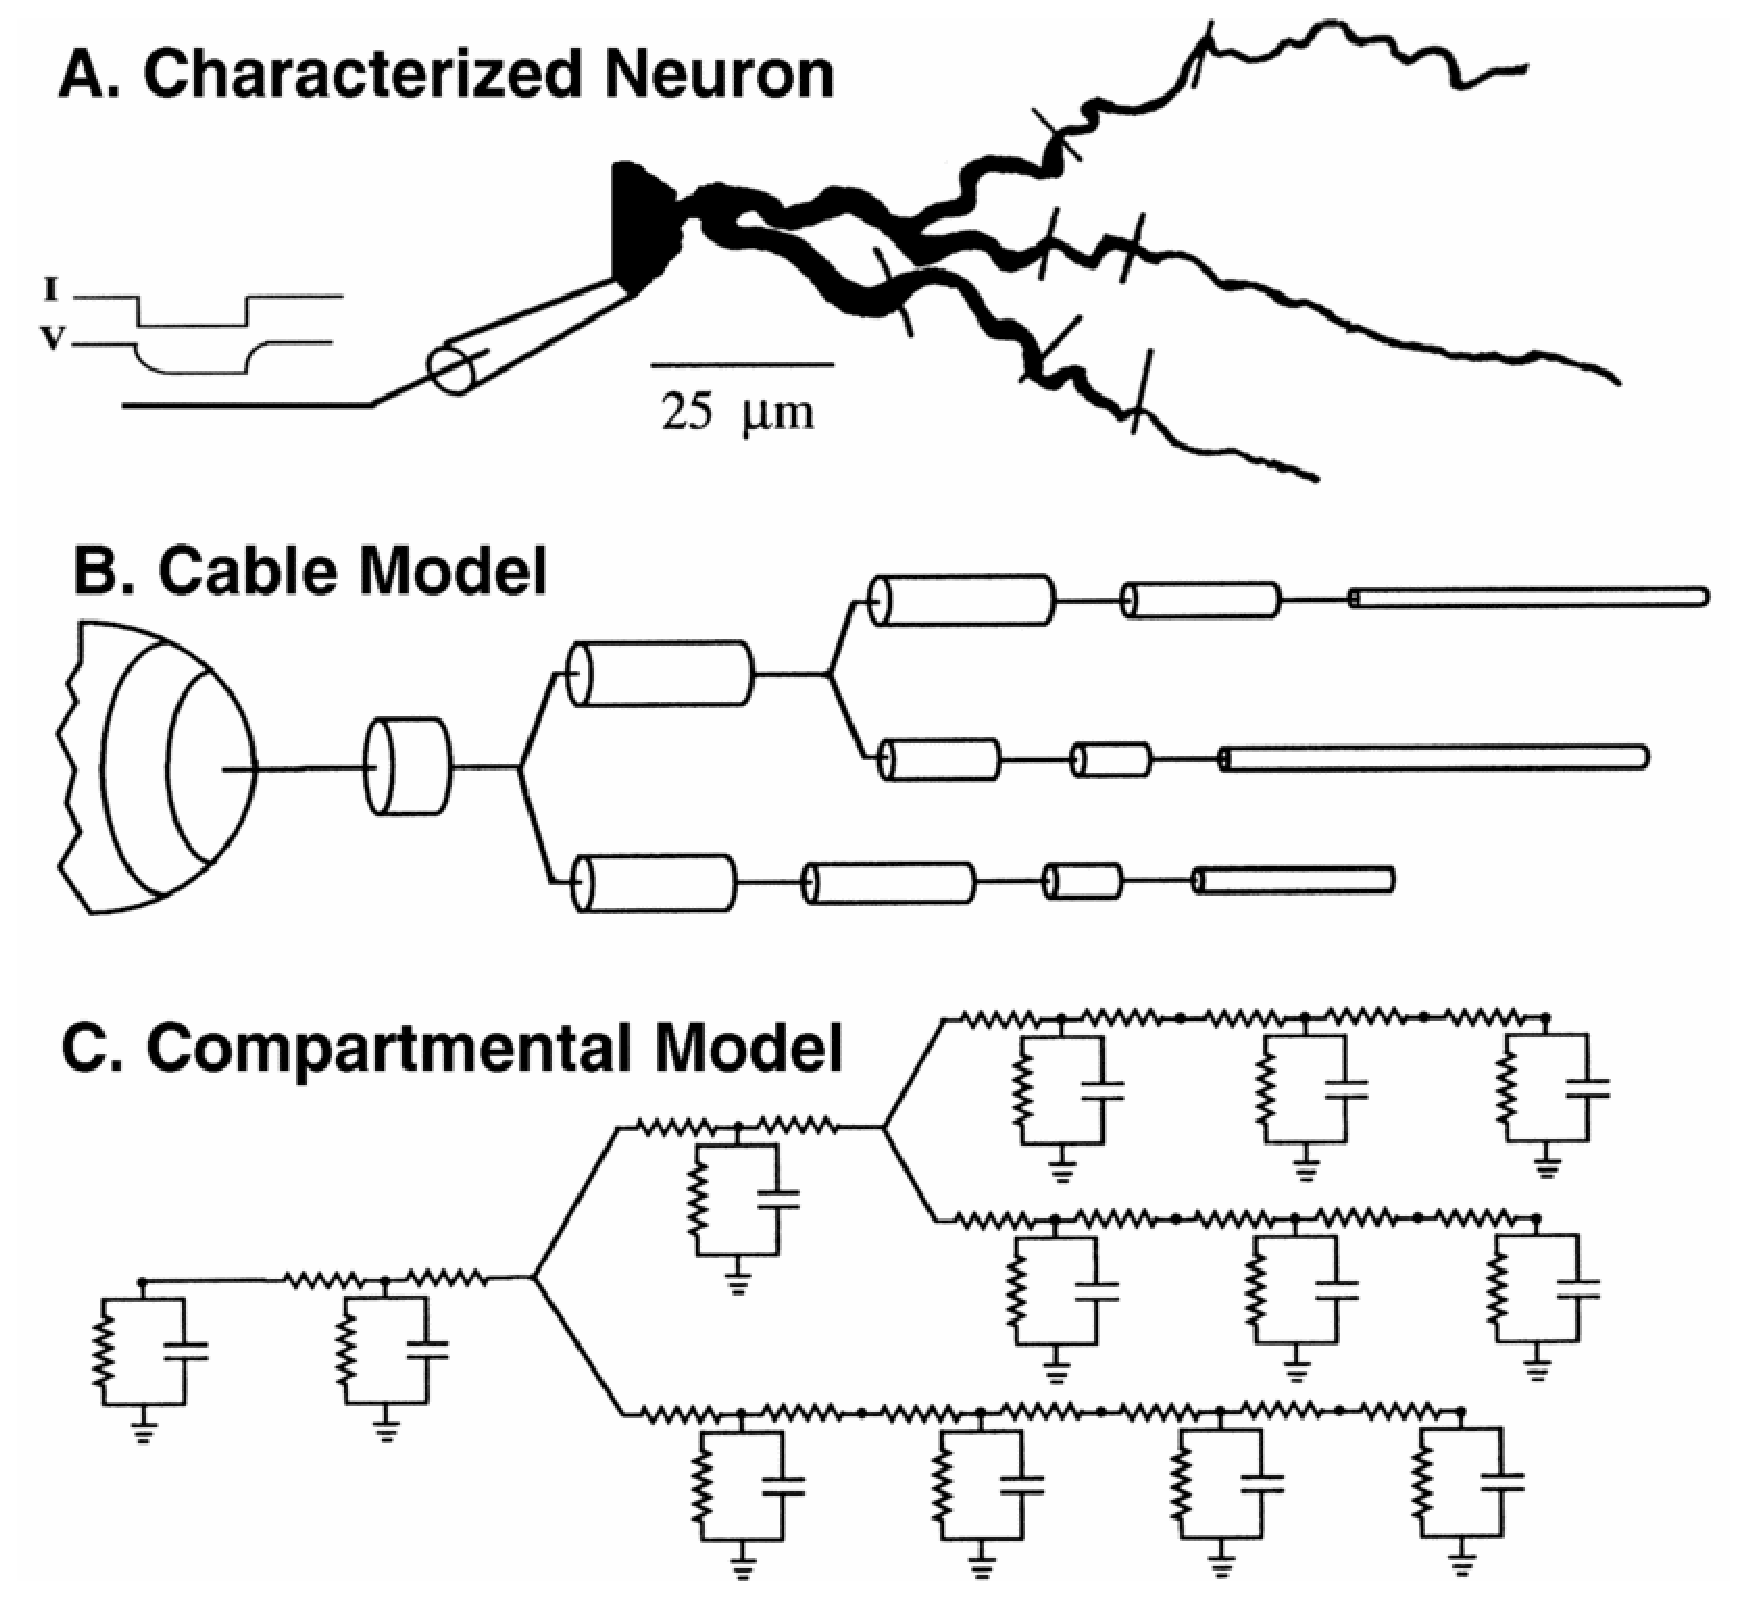
\includegraphics[scale=0.4]{figures/BoGfig5_4s.eps}
  %\caption{enumerate}
  \label{fig:equivcable}
\end{figure}

Equation 5.13 in the BoG gives the attenuation of voltage with distance $x$ along an infinitely long uniform section of dendrite, in terms of the ``space constant" (or ``length constant"), which is given in Equation 5.7. Together, they give:

\begin{displaymath} V(x) = V_0 e^{-x/\lambda}, \mbox{ where } \lambda = \sqrt{(d/4)R_M/R_A} \end{displaymath}

This result is useful for determining the length of the compartments that are used to model a section of dendrite. Sections of dendrite that have a continuous variation of voltage along the length are being replaced by a ``lumped parameter model" with discrete jumps in membrane potential. By using very many short compartments, the compartmental model can approach the result of the continous cable equation. But, for computational efficiency, one would like to use fewer compartments with a length that gives reasonable accuracy. A common guideline used by modelers is to use a compartment length that is less than 1/20 of the space constant. In that case, the voltages in two adjacent compartments will differ by a factor of $e^{-0.05}$ = 0.9512, or by about 5\%.

\subsection*{Determining values of $C_M$, $R_M$, and $R_A$}

Usually one assumes that the values of $C_M$, $R_M$, and $R_A$ are the same in all compartments, as they are intrinsic properties of the neural membrane and cytoplasm. $C_M$ depends on the intrinsic properties of the thickness and dielectric constant of the membrane, and is usually close to 0.01\,$F/m^2$.

Part A of the figure above shows a current injection pulse being injected into the soma of the neuron, and the meaured change in membrane potential. Can you guess why it is a hyperpolarizing pulse, and not a depolarizing one?

Two quantities may be calculated from this measurement, the membrane time constant ($\tau_m$) and the membrane resistance ($R_M$). The membrane time constant for a short uniform section of dendrite is

\begin{displaymath}
	\tau_m = R_mC_m = R_M C_M
\end{displaymath}

Note that it is independent of the dimensions of the section, because $R_m$ is inversely proportional to the surface area, and $C_m$ is proportional to the surface area. This has importance for determining the time that it takes for ionic currents to produce changes in the membrane potential, and is also a measurement that can be made to estimate values for $R_M$.

If the neuron were a simple spherical soma with little dendritic structure, it could be modeled with a single compartment, and the decay of the voltage after the current pulse would be given by an exponential involving the membrane time constant.

\begin{displaymath}
	V(t) = V(0) e^{-t/\tau_m}
\end{displaymath}

so it should be a simple matter to measure the membrane time constant and to estimate $R_M$. The situation is more complicated for long cables or branched dendritic structures, but BoG Section 5.4.2 describes how the solution to the cable equation in the more general case can be expressed in terms of a sum of exponentials with different time constants (Eq. 5.20) and that the longest time constant in the series is just the membrane time constant, $R_M\cdot C_M$.

This can be illustrated with the GENESIS Cable tutorial simulation, which allows one to construct an extensible neuronal cable. Current injection or synaptic input may be provided to any one of the compartments, and all relevant parameters are adjustable from ``pop-up" menus. In the figure below, a passive cable was created with a soma and 10 identical dendrite compartments. A 50 picoampere current injection pulse was applied to the soma, and the resulting membrane potential and its natural log were plotted for the soma and the most distal dentrite compartment

\begin{figure}[h]
\centering
\begin{minipage}{0.5\textwidth}
%{\bf\sf\large A.}
 \centerline{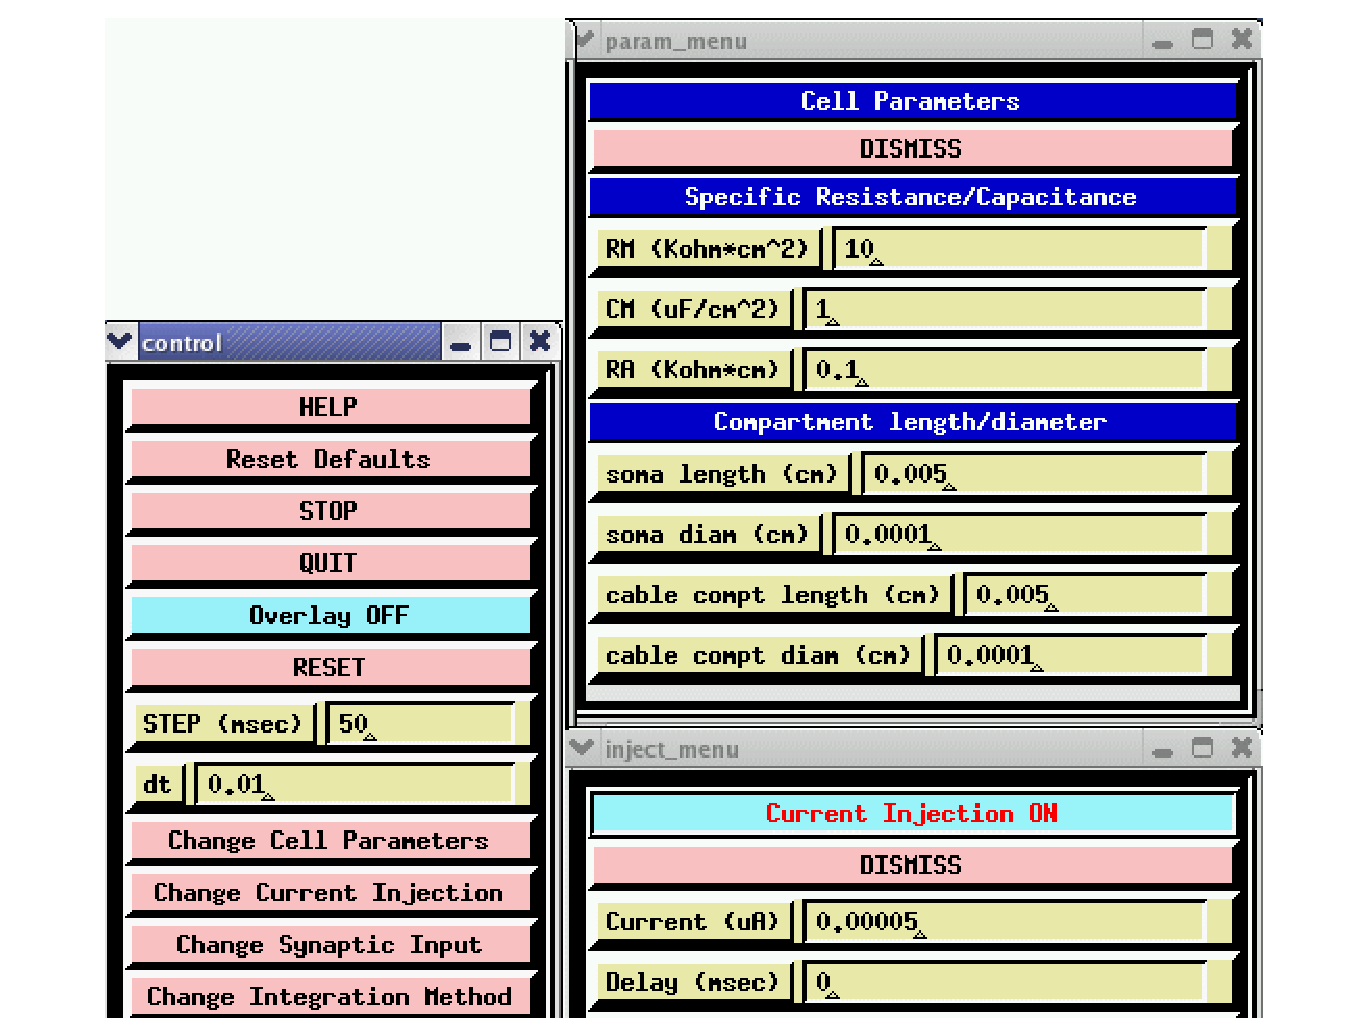
\includegraphics[scale=0.38]{figures/cable1-inj5.eps}}
  %\caption{}
  \end{minipage}
\begin{minipage}{0.45\textwidth}
%{\bf\sf\large B.}
 \centerline{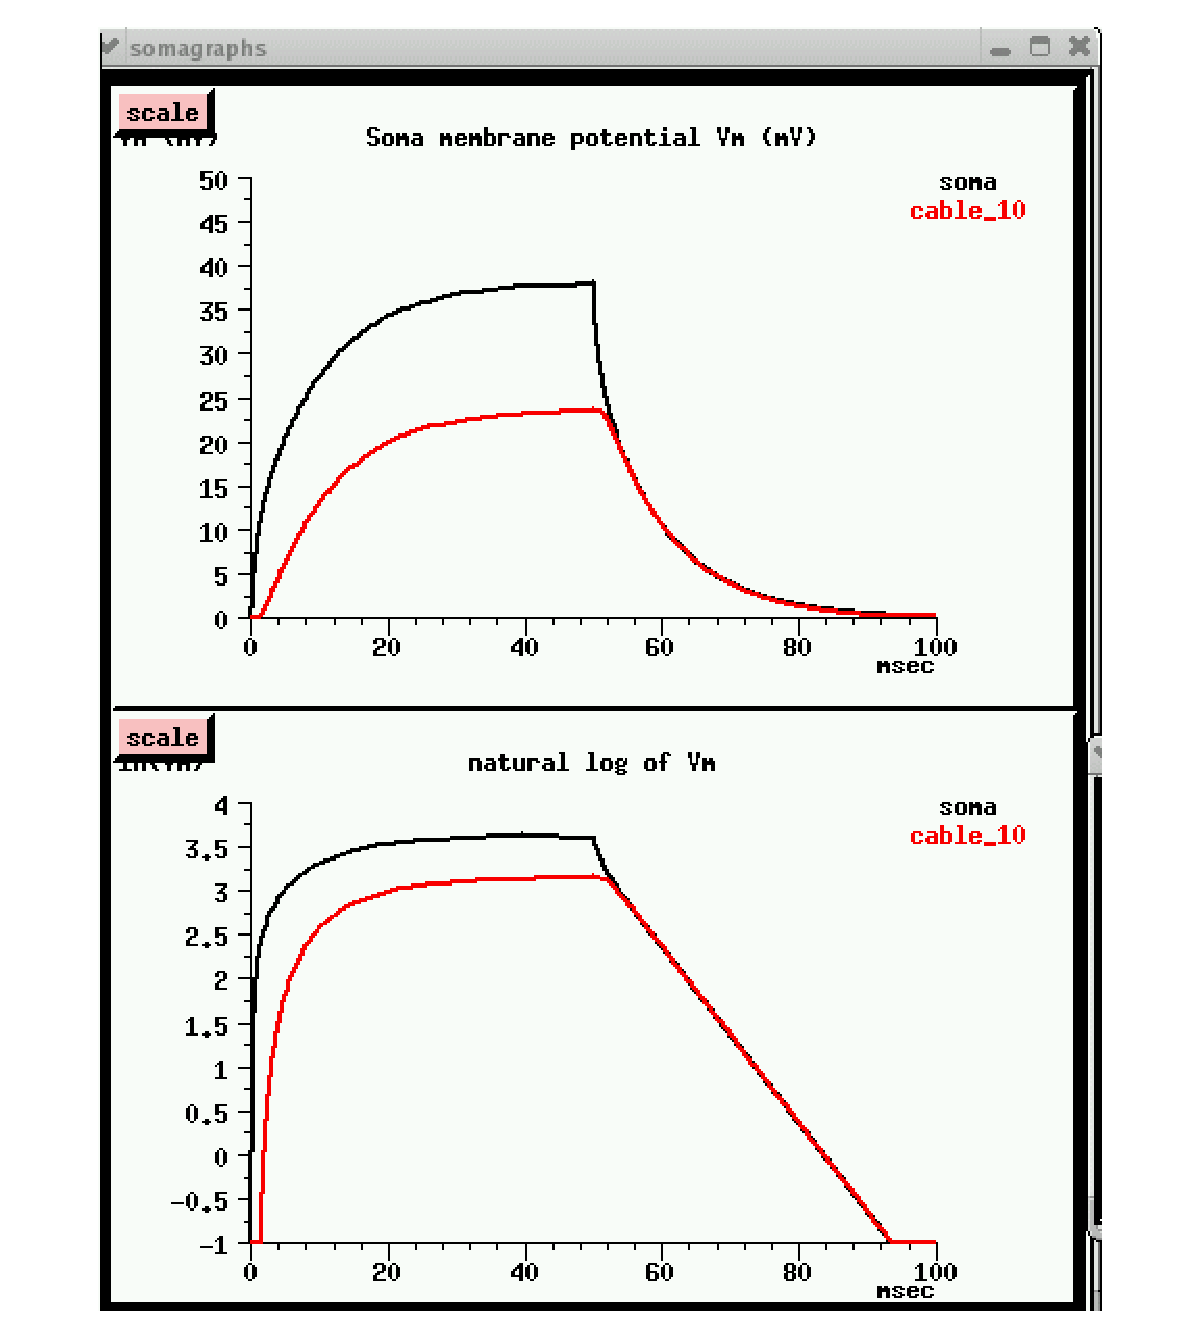
\includegraphics[scale=0.3]{figures/cable2-inj5.eps}}
  %\caption{}
  \end{minipage}
  \label{fig:cableinj}
\end{figure}

Note that the log plot in the lower right graph above becomes linear at longer times, when the term in the series with the largest time constant dominates. From the slope of this line, you should be able to calculate that the membrane time constant $\tau_m$ is about 10\,$msec$, which is the value of $R_M\cdot C_M$. These plots will also let you calculate the voltage attenuation with distance, and compare it with the predicted results for an infinitely long cable using the value of the space constant $\lambda$ and the parameter values that are shown above.

The input resistance of a neuron at the point of a current injection pulse is given by Ohm's law from the change in membrane potential after it has reached a steady state

\begin{displaymath}
	R_{in} = \frac{\Delta V}{\Delta I}.
\end{displaymath}

What is the input resistance of this cable, as measured at the soma? This is another measureable quantity that can help to provide values for $R_M$ and $R_A$. If we were dealing with a neuron that could be modeled as a single soma compartment, then the input resistance would simply be given by the membrane resistance, $R_{in} = R_m = R_M/$area. When there are other compartments, then the axial resistances and membrane resistances of these compartments also add to the resistive load, and the expression becomes more complicated. For a simple model with a few compartments, circuit theory can be used to calculate $R_{in}$ in terms of $R_M$, $R_A$, and the compartment dimensions. BoG Section 5.4.4 gives the result for an infinite cable (Equation 5.24) and a finite cable (Equation 5.26), and discusses conditions under which a branched dendritic structure can be approximated by a single finite cable. This is useful when constructing simple ``ball and stick" models of neurons with a soma having the appropriate surface area of the actual cell soma, connected to a linear chain of cylindrical dendrite compartments. These are designed to provide a ``collapsed dentritic tree" or ``equivalent cable'' with the same passive properties of a much more detailed model made from a reconstruction of a measured cell morpholgy.

However, this is not of much help when dealing with a detailed morphologically accurate model, such as the De Schutter and Bower (1994) Purkinje cell model. The figure below shows a run of the GENESIS Purkinje cell tutorial simulation, with a current injection pulse applied to the soma. The plots were performed in overlay mode to show the results of both a depolarizing pulse of 1\,nA, and a hyperpolarizing pulse of -1\,nA.

\begin{figure}[h]
  \centering
 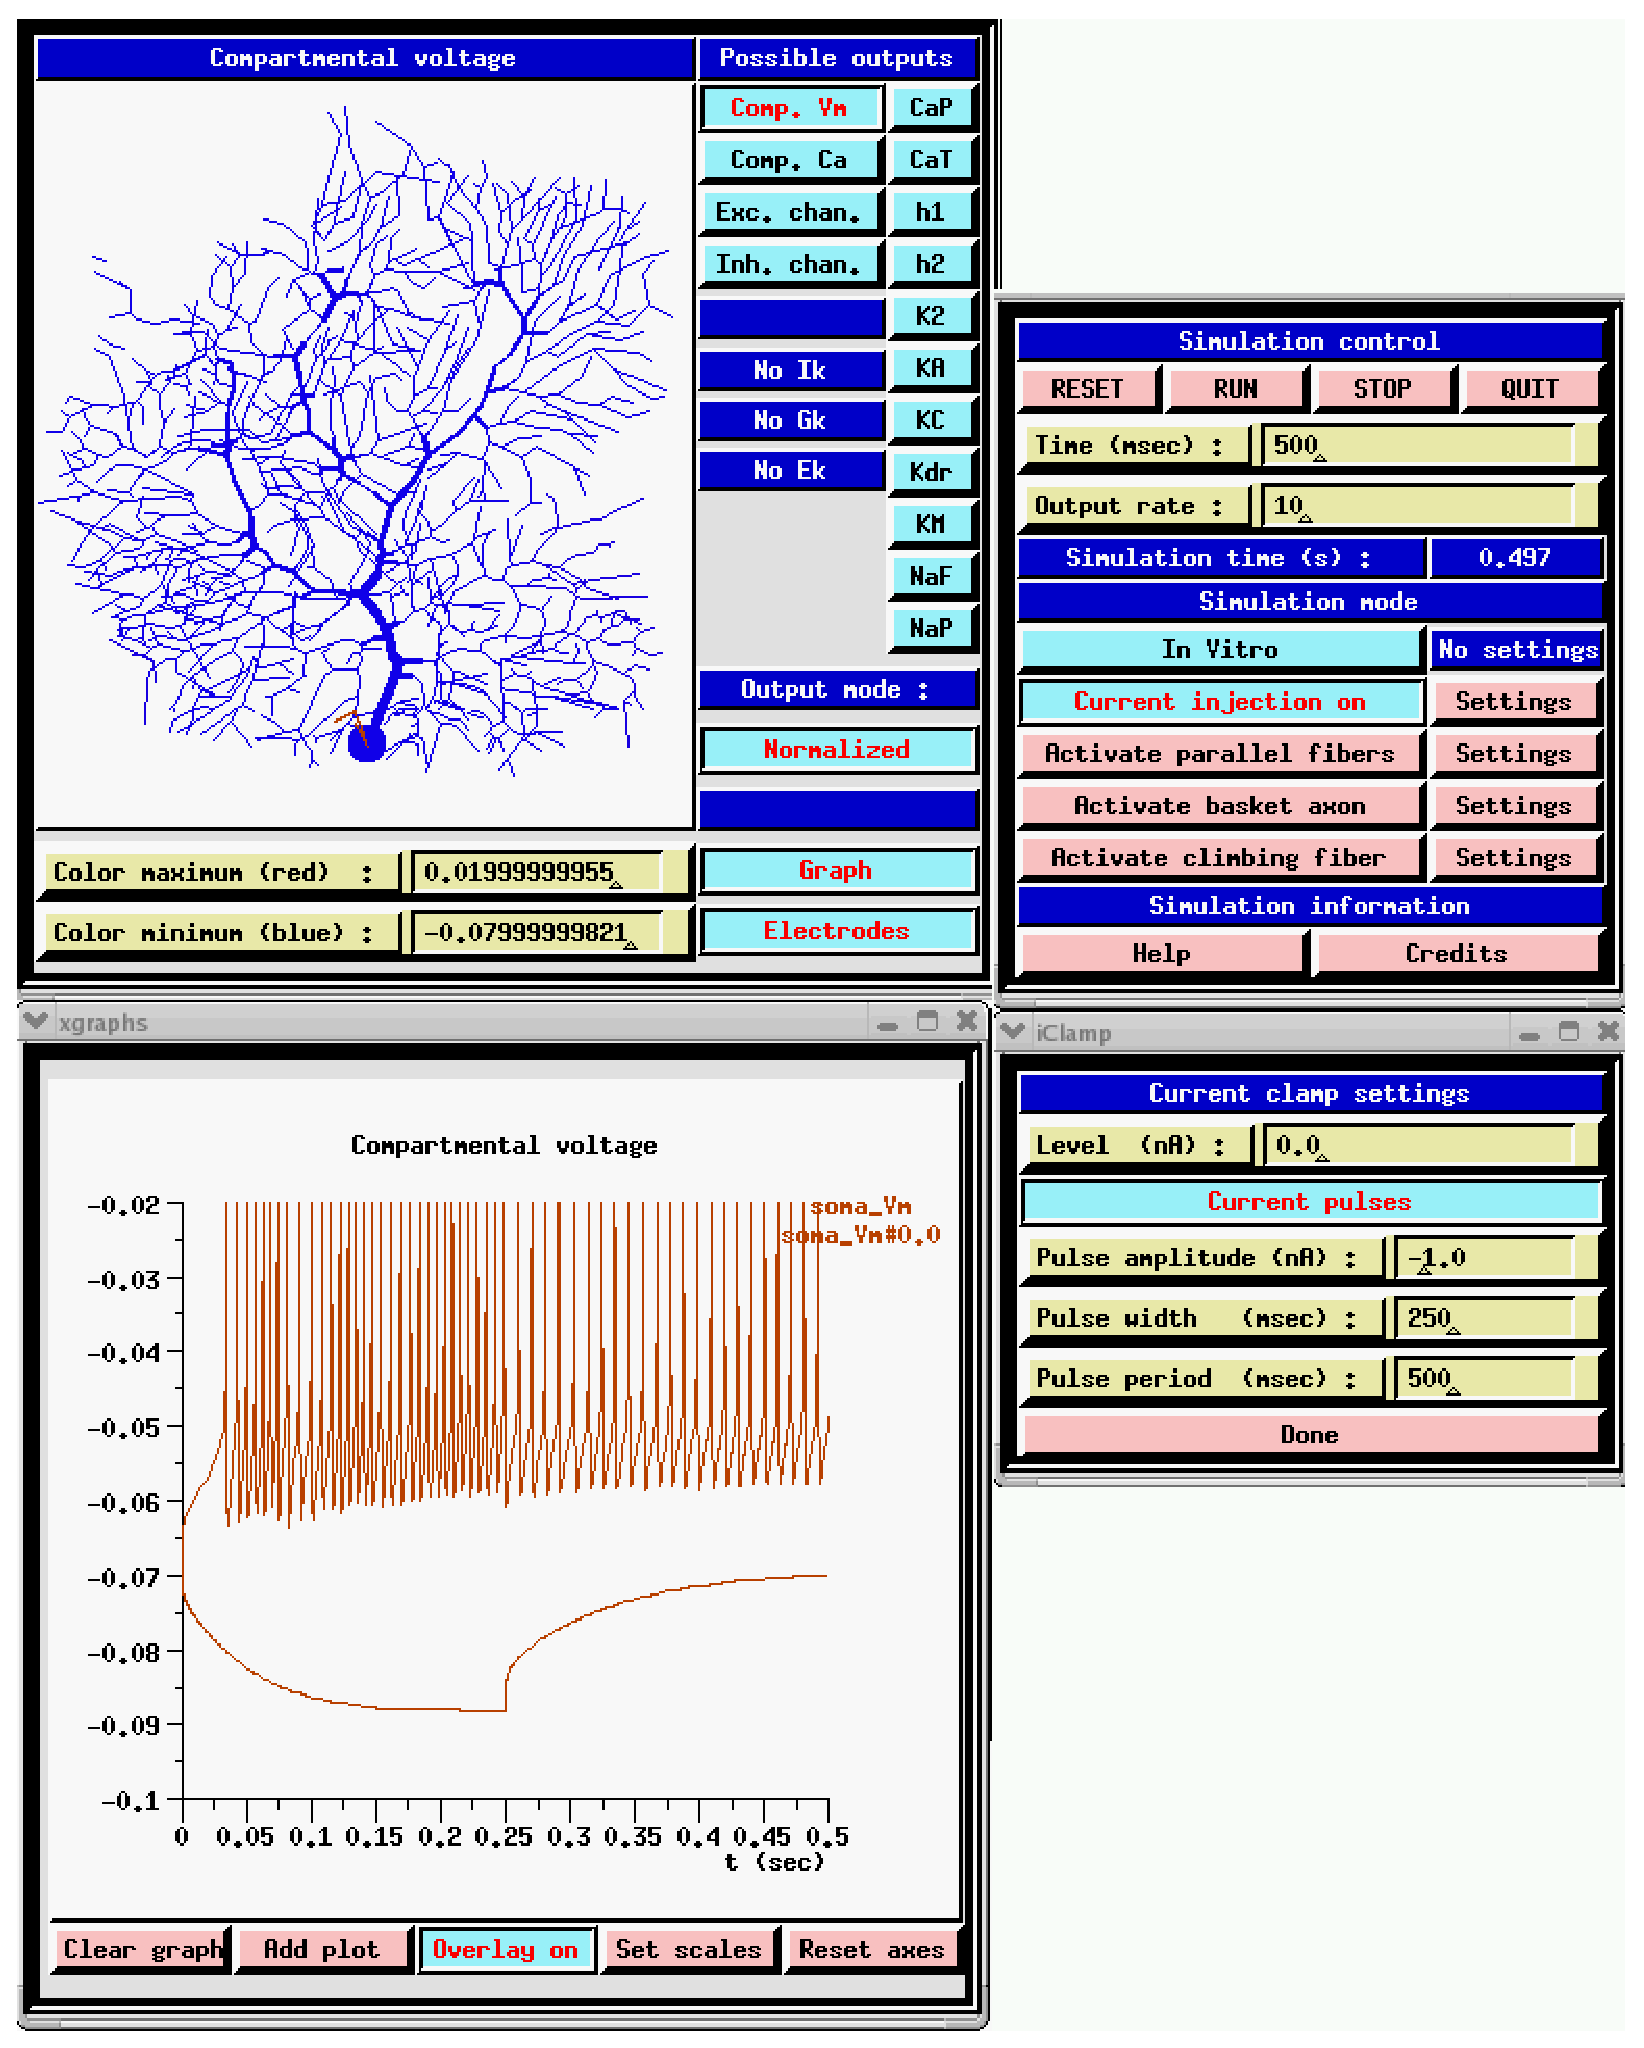
\includegraphics[scale=0.38]{figures/purk_inj5.eps}
  %\caption{enumerate}
  \label{fig:purkinj5}
\end{figure}

Now, is it clear why hyperpolarizing pulses are used? The depolarizing pulse causes the the voltage-activated channels to open, causing the cell to fire. The hyperpolarizing pulse deactivates the channels, and allows one to see the passive properties. (Even this may not be enough to completely get rid of the effects of active channels. Often one applies channel blockers to block any channels that are active at low membrane potentials.) What is the input resistance of this neuron? When fitting parameters for a model of this complexity, it is common to inject current pulses of various amplitudes into the neuron being modeled while recording the membrane potential. The simulation is then run under similar conditions, and automated parameter searches are performed to adjust $C_M$, $R_M$, and $R_A$ to give the best fit of the simulated $V_m$ with the experimental results.

Further details of the process of constructing realistic single cell models are given in a tutorial paper by \href{../tutorial-jaeger/tutorial-jaeger.pdf}{Jaeger (2005)}.

\subsection*{Modeling Synapses}

The next step is to model synaptically (chemically) activated channels. The variable conductance in the generic compartment diagram could also represent a synaptically activated conductance, usually in a dendritic compartment.

\begin{figure}[h]
  \centering
 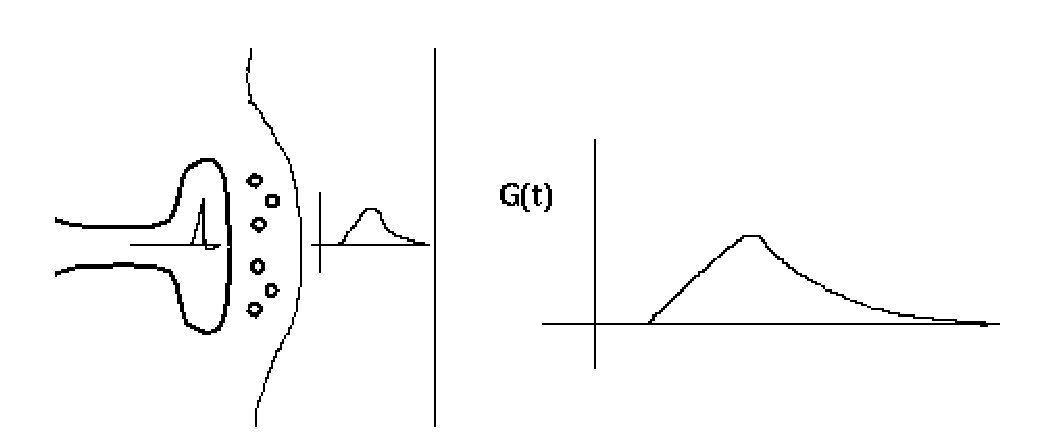
\includegraphics[scale=0.5]{figures/syncond.eps}
  %\caption{enumerate}
  \label{fig:purkinj5}
\end{figure}

This diagram shows a synapse with an action potential propagating to the pre-synaptic terminal, causing neurotransmitter release, and the resulting post-synaptic conductance change, $G$($t$). Current flow through this conductance can lead to a post-synaptic potential (PSP).

There is a lot of biochemistry and molecular biology involved in this behavior, often involving complicated chains of reactions and ``second messengers". Fortunately, we can often use an empirical fit to the observed behavior, rather than modeling it in detail.

Typically, the conductance change from a quantum of neurotransmitter follows a linear rise and exponential decay, so it is often modeled with a so-called ``alpha" function with a single time constant, $\tau$

\begin{displaymath}
	G_k(t) = g_{max}\frac{t}{\tau}e^{(1-t/\tau)}.
\end{displaymath}

Sometimes, a dual exponential function will be used:


\begin{displaymath}
	G_k(t) = \frac{Ag_{max}}{\tau_1 - \tau_2}(e^{-t/\tau_1} - e^{-t/\tau_2}) \mathrm{~for~} \tau_1 > \tau_2
\end{displaymath}

The current due to this conductance is $I = G\cdot (E_k - V_m)$, which may be into or out of the cell, depending on the size of the ionic equilbrium potential $E_k$, relative to the membrane potential. Here we have adopted the convention that a positive current flows into the cell. Thus, if the $E_k$ is large ($Na$ or $Ca$), the current will be into the cell, and it will be a depolarizing (excitatory) synapse. If it is large and negative ($E_k < V_m$, as for potassium), it will be an inhibitory synapse. So, we can use the same model for both types of synapses.

\subsection*{Modeling axons and axonal connections}

If we were interested in understanding the details of axonal propagation we could model an axon as a series of linked compartments containg Hodgkin-Huxley $Na$ and $K$ conductances. We can model synaptic connections more efficiently if we treat an axon as just a delay line for the propagation of spike events that are triggered by action potentials and that last for a single time step.

\begin{figure}[h]
  \centering
 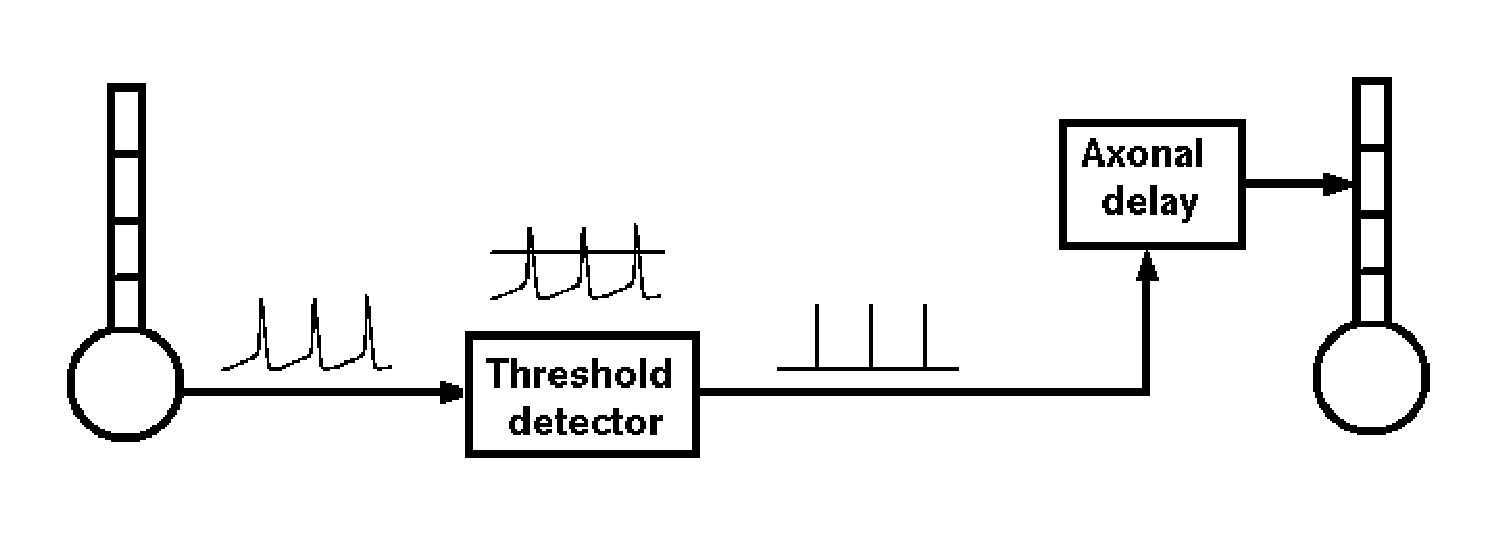
\includegraphics[scale=0.5]{figures/syn-connect.eps}
  %\caption{enumerate}
  \label{fig:synconnect}
\end{figure}

Some simulations demonstrating the effects of synaptic input
We'll use the alpha function form in a GENESIS tutorial simulation called ``Neuron" in order to understand both temporal and spatial summation of synaptic inputs.

Although not done here, this simulation will also let you experiment with ``silent inhibition" (shunting inhibition), in which there can be an inhibitory effect when there is no PSP, or even a slightly depolarizing one. Do you know how this can happen?

Another thing that we can do in this simulation is to scale the conductance by a ``synaptic weight" factor. This would let us experiment with the effect of multiple inputs in synchrony, or with learning (synaptic plasticity) by varying the weight.

Another time constant that is relevant for determining the properties of the cell is the membrane time constant, $R_m\cdot C_m$. This represents the time that it takes to charge up and to discharge the membrane capacitance, and will also affect the duration of a post-synaptic potential. We could also use the Neuron simulation (but won't here) to see what happens if you have a small time constant for synaptic activation and a large membrane time constant.

\end{document}